\section{PMOS threshold}\label{pmos_dimensioning}
Now we take a look at the worst case of 4 stacked PMOS transistors, which is the highest stacking amount which will be possible in technologies relying on this process.

\begin{figure}[H]
	\centering
	\begin{circuitdiagram}{20}{20}
		\power{15}{18.5}{U}{}  % power above pmos
		\wire{15}{18}{15}{16}   % wire above pmos
		\trans{penh}{13}{14}{R}{}{} % pmos -> right
		\Voltarrow{14}{18}{10}{16}{u}{$-V_{GS}$}
		\wire{15}{12}{15}{8}   % wire below pmos
		\resis{15}{5}{V}{$R_D$}{}  % resistor on drain
		\wire{15}{1}{15}{2}   % wire below pmos
		\ground{15}{0.5}{D}  % ground below resistor
		\othersrc[\sigsym{-rec}]{o}{5.5}{15.5}{H}{}{signal}
		\pin{9.5}{15.5}{R}{}	% pin in
		\ground{2.5}{0.5}{D}  % ground below signal source
		\wire{2.5}{1}{2.5}{15.5}   % wire below signal
		\junct{15}{10}   % dot
		\wire{15}{10}{16}{10}   % wire before out
		\pin{17}{10}{R}{out}	% pin out
	\end{circuitdiagram}
	\caption{enhancement-mode PMOS transistor use-case}
\end{figure}

$\approx 4 \mu m$ come mainly from the need to fulfill the condition from \autoref{physics_drive_in}

\begin{equation}
x_e = 2 \cdot \sqrt{D_e \cdot t_e} \gg 2 \cdot \sqrt{D_v \cdot t_v} = x_v
\end{equation}

We already got the background ($N_B \approx 7 \cdot 10^{14} \frac{1}{cm^3}=7 \cdot 10^{20} \frac{1}{m^3}$) concentration from the specs of the basis substrate.

We use a drive in temperature of $1150 \degree C$ which is  $T = 1423.15 \degree K$ in Kelvin which gives us the diffusion coefficient $D=9.1 \cdot 10^{-17}  \frac{m^2}{s}$

Now using
\begin{equation}
N(x,t)
=
\frac{Q}{\sqrt{\pi\cdot D \cdot t}} \cdot \exp\left(\frac{-x^2}{4 \cdot D \cdot t}\right)
\end{equation}

We set the conditions and get the required diffusion time as well as the initial dosage in one shot:
\begin{equation}
N(0,t)
=
\frac{Q}{\sqrt{\pi\cdot D \cdot t}}
=
N_p-N_B
=
7 \cdot 10^{20} \frac{1}{m^3}
\end{equation}
\begin{equation}
x
=
2 \cdot \sqrt{D \cdot t \cdot\ln\left(\frac{N_T}{N_B}\right)}
=
4 \mu m
=
4 \cdot 10^{-6} m
\end{equation}
\begin{equation}
\Rightarrow
t
\approx
16162s
\approx
269min
\approx
\underline{4h 30 min}
\end{equation}
\begin{equation}
\Rightarrow
Q
=
7 \cdot 10^{20} \frac{1}{m^3} \cdot \sqrt{\pi\cdot D \cdot t}
=
7 \cdot 10^{20} \frac{1}{m^3} \cdot \sqrt{\pi} \cdot 2 \cdot 10^{-6} m
\approx
\underline{2.48 \cdot 10^{15} \frac{1}{m^2}}
\end{equation}

\begin{figure}[H]
	\centering
	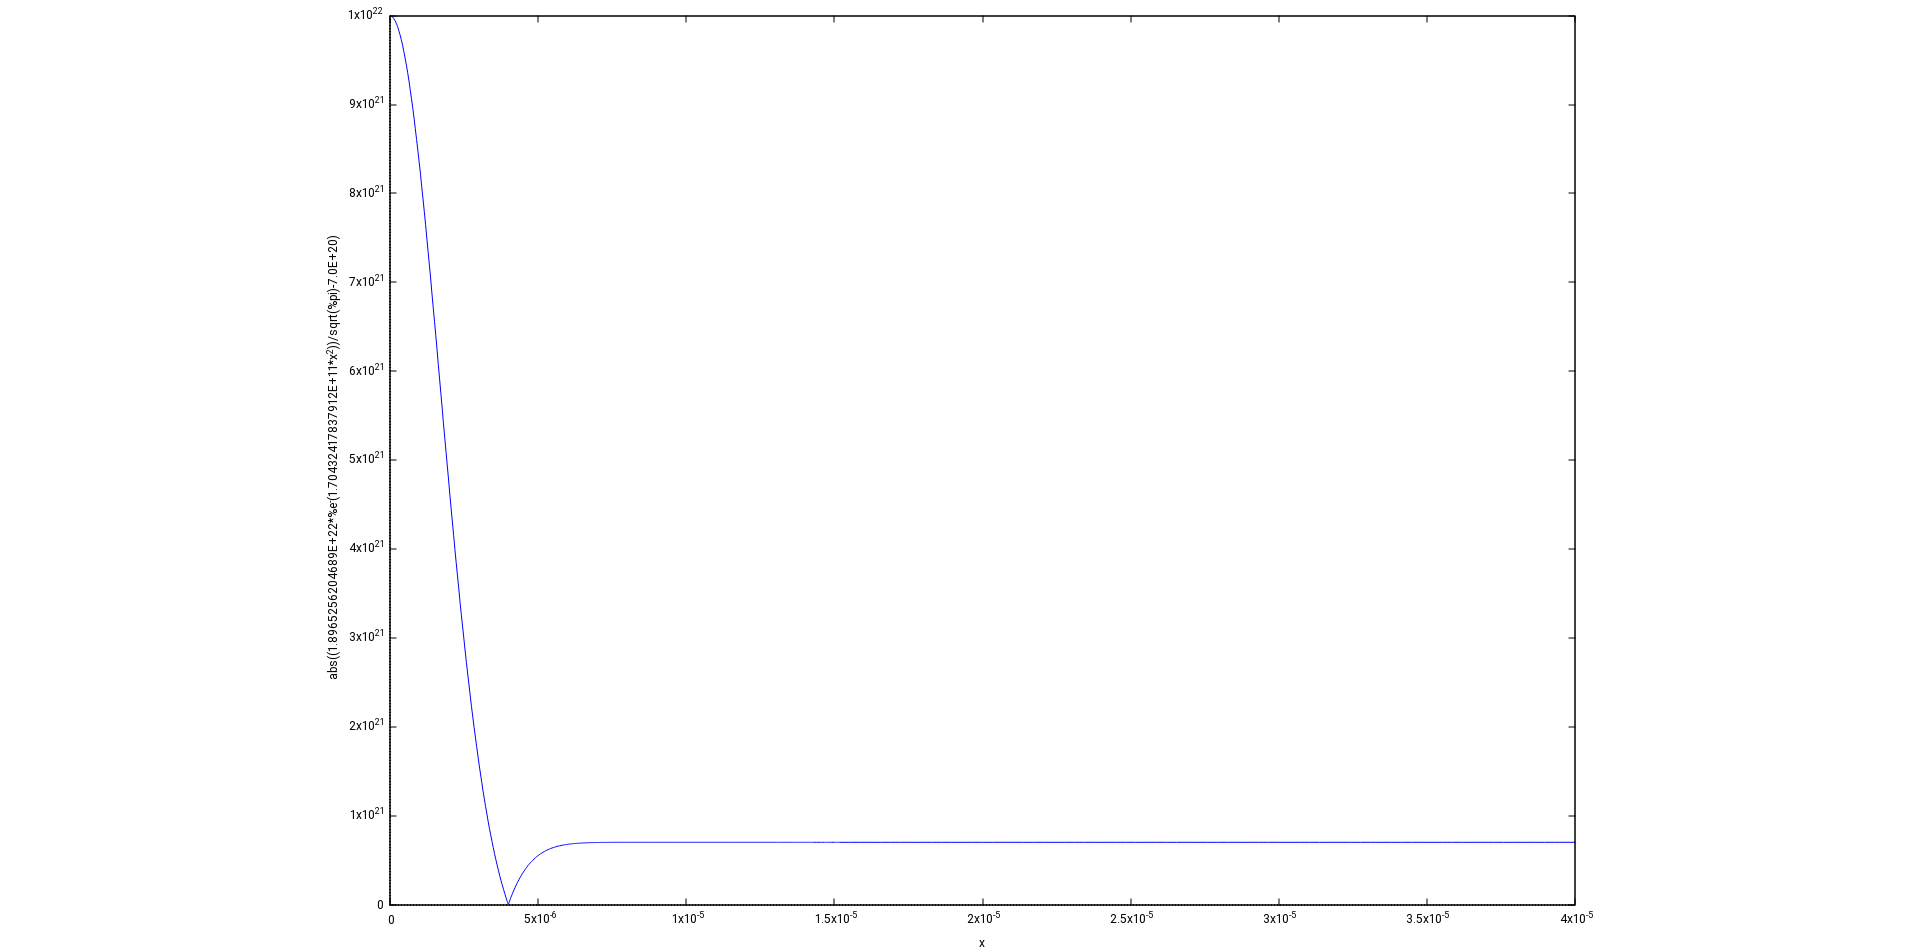
\includegraphics[width=0.75\textwidth]{n-well-diffusion.png}
	\caption{Dopant concentration after 4 hours 30 minutes}
	\label{nwell_drive_in_outcome}
\end{figure}